%%%%%%%%%%%%%%%%%%%%%%%%%%%%%%%%%%%%%%%%%%%%%%%%
%% Compile the master file!
%% 		Slides: Antonio Machicao y Priemer
%% 		Course: Wissenschaftliches Arbeiten
%%%%%%%%%%%%%%%%%%%%%%%%%%%%%%%%%%%%%%%%%%%%%%%%


%%%%%%%%%%%%%%%%%%%%%%%%%%%%%%%%%%%%%%%%%%%%%%%%%%%%
%%%             Metadata                         
%%%%%%%%%%%%%%%%%%%%%%%%%%%%%%%%%%%%%%%%%%%%%%%%%%%%  

\title{
	\LaTeX\ for Linguists
}

\subtitle{\LaTeX\ 3: Graphics, tables \& floats}

\author[aMyP]{
	{\small Sebastian Nordhoff \& Antonio Machicao y Priemer}
	\\
	{\footnotesize \url{www.linguistik.hu-berlin.de/staff/amyp}}
	%	\\
	%	{\footnotesize \href{mailto:mapriema@hu-berlin.de}{mapriema@hu-berlin.de}}
}

\institute{LOT 2019, Amsterdam}

%\date{ }

%\publishers{\textbf{6. linguistischer Methodenworkshop \\ Humboldt-Universität zu Berlin}}

%\hyphenation{nobreak}


%%%%%%%%%%%%%%%%%%%%%%%%%%%%%%%%%%%%%%%%%%%%%%%%%%%%
%%%             Preamble's End                   
%%%%%%%%%%%%%%%%%%%%%%%%%%%%%%%%%%%%%%%%%%%%%%%%%%%%      


%%%%%%%%%%%%%%%%%%%%%%%%%%%%%%%%%%%
%%%%%%%%%%%%%%%%%%%%%%%%%%%%%%%%%%%    
%% Title slide 
\begin{frame}
  \HUtitle
\end{frame}


%% Contents slide
\frame{
\begin{multicols}{2}
	\frametitle{Contents}
%	\tableofcontents[hideallsubsections]
	\tableofcontents
	%[pausesections]
\end{multicols}
	}


%%%%%%%%%%%%%%%%%%%%%%%%%%%%%%%%%%%%
%%%%%%%%%%%%%%%%%%%%%%%%%%%%%%%%%%%%
%% Extra literature

\nocite{Freitag&MyP15a}
\nocite{Knuth1986}
\nocite{Kopka94a}
\nocite{MyP17c}
\nocite{MyP&Kerkhof16a}
	
%%%%%%%%%%%%%%%%%%%%%%%%%%%%%%%%%%%%
%%%%%%%%%%%%%%%%%%%%%%%%%%%%%%%%%%%%


%%%%%%%%%%%%%%%%%%%%%%%%%%%%%%%%%%%%%
%%%%%%%%%%%%%%%%%%%%%%%%%%%%%%%%%%%%%
%%%% Basic literature for these slides
%
%\begin{frame}
%\frametitle{Grundlage \& empfohlene Lektüre}
%
%\dots basierend auf \citet{Freitag&MyP15a} und auf \citet{MyP&Kerkhof16a}\\
%\ras \href{https://www.researchgate.net/publication/279514740_LATEX-Einfuhrung_fur_Linguisten}{LINK}
%
%
%\nocite{Kopka94a}
%
%\end{frame}


%%%%%%%%%%%%%%%%%%%%%%%%%%%%%%%%%%
%%%%%%%%%%%%%%%%%%%%%%%%%%%%%%%%%%
\section{Graphics}
\frame{
\begin{multicols}{2}
\frametitle{~}
	\tableofcontents[currentsection,hideallsubsections]
\end{multicols}
}
%%%%%%%%%%%%%%%%%%%%%%%%%%%%%%%%%%


%%%%%%%%%%%%%%%%%%%%%%%%%%%%%%%%%%
%%%%%%%%%%%%%%%%%%%%%%%%%%%%%%%%%%
\subsection{Including a graphic}
%\frame{
%	%\frametitle{~}
%	\begin{multicols}{2}
%		\tableofcontents[currentsection,hideallsubsections]
%	\end{multicols}
%}
%%%%%%%%%%%%%%%%%%%%%%%%%%%%%%%%%%

\begin{frame}[fragile]
\frametitle{Including a graphic}


\begin{itemize}
	\item Load the \textbf{package} \ltxterm{graphicx}: \lstinline|\usepackage{graphicx}|
	
%\begin{lstlisting}
%\usepackage{graphicx}
%\end{lstlisting}
	
	\item To include the graphic, use the following command (\textbf{file ending}, \ie \ltxpack{.pdf}, doesn't need to be added) :
	
\begin{lstlisting}
\includegraphics[size of graphic]{path/name of graphic}  
\end{lstlisting}

\end{itemize}

\pause
	
%\textbf{Example:}


\includegraphics{../../texfiles-beamer/tex-material/WissArb-latex/LaTeX-flowchart-1.pdf}   

\begin{lstlisting}
\includegraphics{LaTeX-flowchart-1.pdf}    
\end{lstlisting}


\end{frame}

%%%%%%%%%%%%%%%%%%%%%%%%%%%%%%%%%%
%%%%%%%%%%%%%%%%%%%%%%%%%%%%%%%%%%
\subsection{Rescaling the graphic}
%\frame{
%	%\frametitle{~}
%	\begin{multicols}{2}
%		\tableofcontents[currentsection,hideallsubsections]
%	\end{multicols}
%}
%%%%%%%%%%%%%%%%%%%%%%%%%%%%%%%%%%%
\begin{frame}[fragile]
\frametitle{Rescaling the graphic}

Rescaling \textbf{relative} to the \textbf{original size} with the option \lstinline|scale| (\lstinline|scale=0.5| $=$ 50\,\% of the original size)

\begin{lstlisting}
\includegraphics[scale=0.5]{LaTeX-flowchart-1.pdf}  
\end{lstlisting}

\includegraphics[scale=0.5]{../../texfiles-beamer/tex-material/WissArb-latex/LaTeX-flowchart-1.pdf}


\end{frame}


%%%%%%%%%%%%%%%%%%%%%%%%%%%%%%%%%%
\begin{frame}[fragile]
\frametitle{Rescaling the graphic}

Rescaling with \textbf{absolute specification} 


\begin{lstlisting}
\includegraphics[width=5cm]{LaTeX-flowchart-1.pdf}
\includegraphics[height=5cm]{LaTeX-flowchart-1.pdf}
\end{lstlisting}

\includegraphics[width=5cm]{../../texfiles-beamer/tex-material/WissArb-latex/LaTeX-flowchart-1}

Rescaling \textbf{relative} to the \textbf{document size}

\begin{lstlisting}
\includegraphics[width=\linewidth]{LaTeX-flowchart-1.pdf}  
\includegraphics[width=.2\linewidth]{LaTeX-flowchart-1.pdf}
\includegraphics[width=.2\textwidth]{LaTeX-flowchart-1.pdf}
\end{lstlisting}

%\includegraphics[width=.2\textwidth]{../../texfiles-beamer/tex-material/WissArb-latex/LaTeX-flowchart-1.pdf}

\includegraphics[width=.2\linewidth]{../../texfiles-beamer/tex-material/WissArb-latex/LaTeX-flowchart-1}
\end{frame}


%%%%%%%%%%%%%%%%%%%%%%%%%%%%%%%%%%
%%%%%%%%%%%%%%%%%%%%%%%%%%%%%%%%%%
\subsection{Formats and paths}
%\frame{
%	%\frametitle{~}
%	\begin{multicols}{2}
%		\tableofcontents[currentsection,hideallsubsections]
%	\end{multicols}
%}
%%%%%%%%%%%%%%%%%%%%%%%%%%%%%%%%%%

\begin{frame}[fragile]
\frametitle{Formats and paths}

\begin{itemize}
\item The following \textbf{formats} can be used with Xe\LaTeX\ and PDF\LaTeX :
	\begin{itemize}
	\item \ltxterm{.pdf} (vector graphics)
	\item \ltxterm{.png} (raster graphics)
	\item \ltxterm{.jpg} (raster graphics)
	\item \ltxterm{.eps} (vector graphics) (in Xe\LaTeX\ or with \ltxterm{epstopdf} package in PDF\LaTeX )
	\end{itemize}

\pause 

\item You must specify the place where you have saved the graphic \textbf{starting from the location of your \ltxterm{.tex}-file}.

\begin{enumerate}
	\item Graphic and  \ltxterm{.tex}-file are in the same folder:	
	
	\lstinline|\includegraphics{LaTeX-flowchart-1}|
	
	\item Graphic is in a folder \texttt{graphics}. This folder is in the same folder as your  \ltxterm{.tex}-file: 
	
	\lstinline|\includegraphics{graphics/LaTeX-flowchart-1}|
	
	\item \ltxterm{.tex}-file is in a folder. This folder and your graphic are in the same folder: 
	
	\lstinline|\includegraphics{../LaTeX-flowchart-1}|
\end{enumerate}

\end{itemize}

\end{frame}


%%%%%%%%%%%%%%%%%%%%%%%%%%%%%%%%%
\begin{frame}[fragile]
\frametitle{Exercise}

Go to \url{https://github.com/langsci/latex4linguists/blob/master/2-1.md}\\
and follow the instructions of the first \textbf{three blocks} in your \texttt{.tex} file.

\end{frame}


%%%%%%%%%%%%%%%%%%%%%%%%%%%%%%%%%%
%%%%%%%%%%%%%%%%%%%%%%%%%%%%%%%%%%
\section{Tables}
\frame{
%\frametitle{~}
\begin{multicols}{2}
	\tableofcontents[currentsection,hideallsubsections]
\end{multicols}
}
%%%%%%%%%%%%%%%%%%%%%%%%%%%%%%%%%%

\begin{frame}[fragile]
\frametitle{Tables}

\begin{itemize}
	\item \textbf{environment} for tables: \ltxterm{tabular} 
	\item optional argument for \textbf{position} of table
	\item obligatory argument for \textbf{layout} inside a column
	\item separation of table cells: \& 
	\item End of a row: \textbackslash\textbackslash 
\end{itemize}

%\begin{lstlisting}
%\begin{tabular}[position]{layout}
%...    
%\end{tabular}
%\end{lstlisting}

\pause 

\textbf{Example:}

\begin{multicols}{2}
	
%{\scriptsize
\begin{lstlisting}
sample text	
\begin{tabular}[t]{l|c|r}
0001 & 002 & 03 \\
\hline
0A & 000B & 00C \\
\hline
00i  & 0ii  & 000iii  \\
\end{tabular}
\end{lstlisting}
%}
	
	\columnbreak
	
	%\scalebox{.8}{
sample text	
	\begin{tabular}[t]{l|c|r}
%		\hline
		0001 & 002 & 03 \\
		\hline
		0A & 000B & 00C \\
		\hline
		00i  & 0ii  & 000iii  \\
%		\hline
	\end{tabular}
	%}
\end{multicols}

\end{frame}


%%%%%%%%%%%%%%%%%%%%%%%%%%%%%%%%%%%
%\begin{frame}[fragile]
%
%\begin{itemize}
%	\item possible values for \textbf{option}: \ltxterm{t} (top, (\ref{ex:TabTop})), \ltxterm{b} (bottom, (\ref{ex:TabBot})), or \ltxterm{c} (center, (\ref{ex:TabCent})) -- Default: \ltxterm{c}
%	
%	\begin{exe}
%		\ex\label{ex:TabTop} \ltxterm{t}:		
%		sample text	
%		\begin{tabular}[t]{l|c|r}
%			%		\hline
%			0001 & 002 & 03 \\
%			\hline
%			0A & 000B & 00C \\
%			\hline
%			00i  & 0ii  & 000iii  \\
%			%		\hline
%		\end{tabular}
%	
%\pause 
%	
%		\ex\label{ex:TabBot}  \ltxterm{b}:	
%		sample text	
%		\begin{tabular}[b]{l|c|r}
%			%		\hline
%			0001 & 002 & 03 \\
%			\hline
%			0A & 000B & 00C \\
%			\hline
%			00i  & 0ii  & 000iii  \\
%			%		\hline
%		\end{tabular}
%
%\pause 
%
%		\ex\label{ex:TabCent}  \ltxterm{c}:
%		sample text	
%		\begin{tabular}[c]{l|c|r}
%			%		\hline
%			0001 & 002 & 03 \\
%			\hline
%			0A & 000B & 00C \\
%			\hline
%			00i  & 0ii  & 000iii  \\
%			%		\hline
%		\end{tabular}
%	\end{exe}
%\end{itemize}
%
%\end{frame}


%%%%%%%%%%%%%%%%%%%%%%%%%%%%%%%%%%%
%\begin{frame}[fragile]
%%\frametitle{Tabellen}
%
%Die Option \textbf{Position} kann die Werte \ltxterm{t} (top), \ltxterm{c} (center), oder \ltxterm{b} (bottom) annehmen. 
%Diese Positionswerte geben die \textbf{vertikale Positionierung der gesamten Tabelle in Bezug zur aktuellen Zeile} (zur zuletzt geschriebenen Zeile), die Default-Einstellung ist in diesem Fall \ltxterm{center}.
%
%\begin{multicols}{2}
%
%Code für \textbf{top}:
%
%\columnbreak
%
%{\scriptsize
%	\begin{lstlisting}
%	Hier ist die aktuelle Zeile
%	\begin{tabular}[t]{l|c|r}
%	Zelle 01 & Zelle 02 & Zelle 03 \\
%	\hline
%	Zelle A & Zelle B & Zelle C \\
%	\hline
%	Zelle  & Zelle  & Zelle  \\
%	\end{tabular}
%	\end{lstlisting}
%}
%
%\end{multicols}
%
%Hier ist die aktuelle Zeile	
%\begin{tabular}[t]{l|c|r}
%Zelle 01 & Zelle 02 & Zelle 03 \\
%\hline
%Zelle A & Zelle B & Zelle C \\
%\hline
%Zelle  & Zelle  & Zelle  \\
%\end{tabular}
%
%\end{frame}
%
%
%%%%%%%%%%%%%%%%%%%%%%%%%%%%%%%%%%%
%\begin{frame}[fragile]
%%\frametitle{Tabellen}
%
%\begin{multicols}{2}
%
%Code für \textbf{bottom}:
%
%\columnbreak
%
%{\tiny
%\begin{lstlisting}
%Hier ist die aktuelle Zeile
%\begin{tabular}[b]{l|c|r}
%Zelle 01 & Zelle 02 & Zelle 03 \\
%\hline
%Zelle A & Zelle B & Zelle C \\
%\hline
%Zelle  & Zelle  & Zelle  \\
%\end{tabular}
%\end{lstlisting}
%}
%
%\end{multicols}
%
%Hier ist die aktuelle Zeile	
%\begin{tabular}[b]{l|c|r}
%Zelle 01 & Zelle 02 & Zelle 03 \\
%\hline
%Zelle A & Zelle B & Zelle C \\
%\hline
%Zelle  & Zelle  & Zelle  \\
%\end{tabular}
%
%
%\pause 
%
%
%\begin{multicols}{2}
%
%Code für \textbf{center}:
%
%\columnbreak
%
%{\tiny
%\begin{lstlisting}
%Hier ist die aktuelle Zeile
%\begin{tabular}[c]{l|c|r}
%Zelle 01 & Zelle 02 & Zelle 03 \\
%\hline
%Zelle A & Zelle B & Zelle C \\
%\hline
%Zelle  & Zelle  & Zelle  \\
%\end{tabular}
%\end{lstlisting}
%}
%
%\end{multicols}
%
%
%Hier ist die aktuelle Zeile	
%\begin{tabular}[c]{l|c|r}
%Zelle 01 & Zelle 02 & Zelle 03 \\
%\hline
%Zelle A & Zelle B & Zelle C \\
%\hline
%Zelle  & Zelle  & Zelle  \\
%\end{tabular}
%
%\end{frame}


%%%%%%%%%%%%%%%%%%%%%%%%%%%%%%%%%%%
\begin{frame}[fragile]
%\frametitle{Tabellen}

\begin{itemize}
	\item possible values for the \textbf{obligatory argument}: \ltxterm{l} (left), \ltxterm{c} (centered), \ltxterm{r} (right), \ltxterm{p\{length\}} (fixed width), optionally \ltxterm{|} (pipe, for vertical lines between columns)
	
	\item each column must have an alignment specification (\ie \ltxterm{l}, \ltxterm{c}, \ltxterm{r}, or \ltxterm{p})
	
\end{itemize}

%\pause 

\begin{multicols}{2}

{\scriptsize
\begin{lstlisting}
\begin{tabular}[t]{lc|r|p{1.5cm}}
00001 & 002 & 03 & 0004 \\
\hline
0A & 000B & 00C & 0000D\\
\hline
00i  & 0000ii  & 000iii  & iv\\
\end{tabular}
\end{lstlisting}
}

\columnbreak

%\scalebox{.8}{
\begin{tabular}[t]{lc|r|p{1.5cm}}
	00001 & 002 & 03 & 0004 \\
	\hline
	0A & 000B & 00C & 0000D\\
	\hline
	00i  & 0000ii  & 000iii  & iv\\
\end{tabular}
%}
\end{multicols}

\end{frame}


%%%%%%%%%%%%%%%%%%%%%%%%%%%%%%%%%%%%
%\begin{frame}[fragile]
%%\frametitle{Tabellen}
%
%\begin{itemize}
%\item Tabellen werden Zeile für Zeile geschrieben. 
%
%\item Das \textbf{Et-Zeichen} \ltxterm{\&} trennt zwei Zellen von einander.
%
%\item Der \textbf{doppelte Backslash} \textbackslash\textbackslash\ markiert das Ende einer Zeile.
%
%\end{itemize}
%
%\small{
%\begin{lstlisting}
%Aktuelle Zeile
%\begin{tabular}[c]{lc|rp{1.7cm}|}
%l-bündig & zentriert & r-bündig & feste Breite \\
%\hline
%viel Inhalt & viel Inhalt & viel viel Inhalt & viel viel Inhalt \\
%wenig & & wenig & wenig \\
%\end{tabular}
%\end{lstlisting}
%
%%\outputbox{
%Aktuelle Zeile
%\begin{tabular}[c]{lc|rp{1.7cm}|}
%l-bündig & zentriert & r-bündig & feste Breite \\
%\hline
%viel Inhalt & viel Inhalt & viel viel Inhalt & viel viel Inhalt \\
%wenig & & wenig & wenig \\
%\end{tabular}
%}
%%}
%\end{frame}


%%%%%%%%%%%%%%%%%%%%%%%%%%%%%%%%%%%
\begin{frame}[fragile]
%\frametitle{Tabellen}

Two more helpful commands for tables:

\begin{itemize}
	\item With \lstinline|\multicolumn{number of colums}{alignment}{text}| text can occupy more than one column.
	
	\item With \lstinline|\cline{cell number - cell number}| you can have horizontal lines specifying its begin (cell number) and end (cell number).
\end{itemize}

%\footnotesize{
%Beispiele weiterer Tabellen:

\begin{multicols}{2}

\begin{lstlisting}
\begin{tabular}[t]{llr}
\multicolumn{2}{c}{Item} &  \\
\cline{1-2}
article & unit & price \\
\hline
proofreading & per words & 0.02 \\
layout & per page & 0.80 \\
printing & per page & 0.99 \\
typesetting & per article & 40.33 \\
\end{tabular}
\end{lstlisting}

%\begin{tabular}[t]{llr}
%\multicolumn{2}{c}{Item} &  \\
%article & unit & price \\
%proofreading & per words & 0.02 \\
%layout & per page & 0.80 \\
%printing & per page & 0.99 \\
%typesetting & per article & 40.33 \\
%\end{tabular}
%
%\vspace{\baselineskip}
%
%\begin{tabular}[t]{|l|l|r|}
%\hline
%\multicolumn{2}{|c}{Item} &  \\
%\hline
%article & unit & price \\
%\hline
%proofreading & per words & 0.02 \\
%\hline
%layout & per page & 0.80 \\
%\hline
%printing & per page & 0.99 \\
%\hline
%typesetting & per article & 40.33 \\
%\hline
%\end{tabular}
%
%\vspace{\baselineskip}

\columnbreak{}

\begin{tabular}[t]{llr}
\multicolumn{2}{c}{Item} &  \\
\cline{1-2}
article & unit & price \\
\hline
proofreading & per words & 0.02 \\
layout & per page & 0.80 \\
printing & per page & 0.99 \\
typesetting & per article & 40.33 \\
\end{tabular}

%\vspace{\baselineskip}
%
%\begin{tabular}[t]{llr}
%\toprule
%\multicolumn{2}{c}{Item} &  \\
%\cmidrule{1-2}
%article & unit & price \\
%\midrule
%proofreading & per words & 0.02 \\
%layout & per page & 0.80 \\
%printing & per page & 0.99 \\
%typesetting & per article & 40.33 \\
%\bottomrule
%\end{tabular}

\end{multicols}
%}
\end{frame}


%%%%%%%%%%%%%%%%%%%%%%%%%%%%%%%%%%
\begin{frame}[fragile]

The package \lstinline|\usepackage{tabularx}| provides 
\begin{itemize}
	\item an extra \textbf{argument} to \textbf{specify the width} of the table, and
	
	\item a new column specifier \ltxterm{X}; the \ltxterm{X}-columns will be \textbf{stretched} until the table is as wide as specified.
\end{itemize}

The package \lstinline|\usepackage{booktabs}| provides \lstinline|\toprule|, \lstinline|\bottomrule|, \lstinline|\midrule|, and \lstinline|\cmidrule{x-y}| which are versions of \lstinline|\hline| and \lstinline|\cline{x-y}| with better spacing.

\smallskip

The package 
\lstinline|\usepackage{multirow}| gives you the possibility to merge cells vertically.

\begin{multicols}{2}
	
\begin{lstlisting}
\begin{tabularx}{.4\textwidth}{XXX}
\toprule
0001&002&03\\
\midrule
0A&\multirow{2}{*}{Bii}&000C\\
\cmidrule{1-1}\cmidrule{3-3}
00i& &000iii\\
\bottomrule
\end{tabularx}
\end{lstlisting}
	
	\columnbreak
	
	\begin{tabularx}{.4\textwidth}{XXX}
		\toprule
		0001&002&03\\
		\midrule
		0A&\multirow{2}{*}{Bii}&000C\\
		\cmidrule{1-1}\cmidrule{3-3}
		00i& &000iii\\
		\bottomrule
	\end{tabularx}
	
\end{multicols}

\end{frame}


%%%%%%%%%%%%%%%%%%%%%%%%%%%%%%%%%%
%%%%%%%%%%%%%%%%%%%%%%%%%%%%%%%%%%
\section{Floating environments}
\frame{
	%\frametitle{~}
	\begin{multicols}{2}
		\tableofcontents[currentsection,hideallsubsections]
	\end{multicols}
}
%%%%%%%%%%%%%%%%%%%%%%%%%%%%%%%%%%

\begin{frame}[fragile]
\frametitle{Floating environments}

With floating environments, \LaTeX\ puts figures or tables in the best position to avoid gaps in the layout. 


\begin{multicols}{2}

{\small
\begin{lstlisting}
It is not necessary that this text has 
any meaning.
\begin{table}[htb]
\centering

\begin{tabular}[t]{l|l}
Eins & Zwei \\
\hline
Drei & Vier \\
\end{tabular}

\caption{Caption of my table}
\label{fig:TableFloat}
\end{table}
\end{lstlisting}
}

\columnbreak

It is not necessary that this text has any meaning.
\begin{table}[htb]
	\centering
	
	\begin{tabular}[t]{l|l}
		Eins & Zwei \\
		\hline
		Drei & Vier \\
	\end{tabular}
	
	\caption{Caption of my table}
	\label{fig:TableFloat}
\end{table}

\end{multicols}

\end{frame}


%%%%%%%%%%%%%%%%%%%%%%%%%%%%%%%%%%%
\begin{frame}[fragile]
%\frametitle{Gleitumgebung}

\begin{itemize}
	\item floating for tables: \lstinline|table|
	
	\item floating for figures: \lstinline|figure|
	
	\item In the environment, the command \lstinline|\caption{ }| can be used.
	
	\item Optionally, preferences for the position can be given: \ltxterm{h} (here), \ltxterm{t} (top), \ltxterm{b} (bottom), \ltxterm{p} (new page).
	
	\item Inside the environment, you can specify the position of the figure/table
\end{itemize}	

\begin{multicols}{2}
	
\begin{lstlisting}
\begin{figure}[htb]
\centering

\includegraphics{LaTeX-flowchart-1.pdf}
\caption{My first float}
\label{fig:FigFloat}
\end{figure}
\end{lstlisting}

\columnbreak

\begin{figure}[htb]
%\centering
\includegraphics[scale=0.5]{../../texfiles-beamer/tex-material/WissArb-latex/LaTeX-flowchart-1.pdf}
\caption{My first float}
\label{fig:FigFloat}
\end{figure}
\end{multicols}

\end{frame}


%%%%%%%%%%%%%%%%%%%%%%%%%%%%%%%%%
\begin{frame}[fragile]
\frametitle{Exercise}


Go to \url{https://github.com/langsci/latex4linguists/blob/master/2-1.md}\\
and follow the instructions of \textbf{all blocks} in your \texttt{.tex} file.

%Download the PDF \alert{\texttt{myDocument-EX4.pdf}} and replicate it with the commands you have already learnt. Follow the instructions in the last section and install the packages.

\end{frame}


%%%%%%%%%%%%%%%%%%%%%%%%%%%%%%%%%%%
%%%%%%%%%%%%%%%%%%%%%%%%%%%%%%%%%%%
%\section{XY}
%%\frame{
%%\begin{multicols}{2}
%%\frametitle{~}
%%	\tableofcontents[currentsection]
%%\end{multicols}
%%}
%%%%%%%%%%%%%%%%%%%%%%%%%%%%%%%%%%%
%
%\begin{frame}{XY}
%
%\begin{itemize}
%	\item XY
%\end{itemize}
%
%\end{frame}


%%%%%%%%%%%%%%%%%%%%%%%%%%%%%%%%%%%%
%%%%%%%%%%%%%%%%%%%%%%%%%%%%%%%%%%%%
%\iftoggle{handout}{
%%% BEGIN handout true
%
%%%%%%%%%%%%%%%%%%%%%%%%%%%%%%%%%%%%
%	
%%Test Toggle ON
%
%}
%%% END handout true 
%%% BEGIN handout false
%{
%%%%%%%%%%%%%%%%%%%%%%%%%%%%%%%%%%%%
%
%% Test Toggle OFF
%
%}%% END handout false
%%%%%%%%%%%%%%%%%%%%%%%%%%%%%%%%%%%%